\documentclass[a4paper,slidestop,xcolor=pst,blue]{beamer}

\input{slidesHeader.tex}

\title[Capa de Persistencia]{Capa de Persistencia}

\author[P. S{\'a}nchez]{\alert{Pablo S{\'a}nchez}}

\institute[IIE]{
		   Dpto. Ingenier{\'i}a Inform{\'a}tica y Electr{\'o}nica \\
		   Universidad de Cantabria \\
		   Santander (Cantabria, Espa{\~n}a) \\
		   \texttt{p.sanchez@unican.es}
}

\date{}

\begin{document}

\begin{frame}[c]
	\titlepage
	\begin{columns}
		\column{0.50\linewidth}
			\centering
    		\includegraphics[width=.28\textwidth,keepaspectratio=true]{images/istr.eps}
		\column{0.50\linewidth}
			\centering
			\includegraphics[width=.25\textwidth,keepaspectratio=true]{images/uc.eps}
	\end{columns}
\end{frame}

\begin{frame}[c]
    \frametitle{\alert{Advertencia}}
    \begin{center}
        Todo el material contenido en este documento no constituye en modo alguno una obra de referencia o apuntes oficiales mediante el cual se puedan preparar las pruebas evaluables necesarias para superar la asignatura. \ \\
        \ \\
        Este documento contiene exclusivamente una serie de diapositivas cuyo objetivo es servir de complemento visual a las actividades realizadas en el aula para la transmisi{\'o}n del contenido sobre el cual versar{\'a}n las mencionadas pruebas evaluables.  \ \\
        \ \\
        Dicho de forma m{\'a}s clara, \alert{estas transparencias no son apuntes y su objetivo no es servir para que el alumno pueda preparar la asignatura.}
    \end{center}
\end{frame}

\section{Introducci�n}

\subsection{Objetivos y Bibliograf�a}

\begin{frame}[c]
    \frametitle{Objetivos del Tema}
    \begin{enumerate}[<+->]
         \item Comprender en profundidad cu�les son las responsabilidades de la capa de persistencia.
         \item Comprender el funcionamiento de los puentes de persistencia de objetos.
         \item Conocer los patrones de persistencia estructurales.
         \item Conocer los patrones de acceso a datos.
         \item Conocer los patrones de control de la concurrencia.
         \item Ser capaz de utilizar JPA para generar esquemas relacionales.
         \item Ser capaz de utilizar repositorios para acceder a datos persistentes.
    \end{enumerate}
\end{frame}

\begin{frame}[c]
    \frametitle{Bibliograf�a}
    \begin{thebibliography}{1}

        \bibitem[Fowler, 2002]{Fowler2002}
        Fowler, M. (2002).
        \newblock {\em {Patterns of Enterprise Application Architecture}}.
        \newblock Addison-Wesley.

        \bibitem[Esposito and Saltarello, 2014]{Esposito2014}
        Esposito, D. y Saltarello, A. (2014).
        \newblock {\em {Microsoft .NET - Architecting Applications for the
          Enterprise}}. 2� Ed..
        \newblock Microsoft Press

        \bibitem[Bauer, 2015]{Bauer2015}
        Bauer, C., King. G. y Gregory G. (2015).
        \newblock {\em {Java Persistence with Hibernate}}. 2� Ed.
        \newblock Manning

        %% JPA

        %% Spring Data

    \end{thebibliography}
\end{frame}

\subsection{Contexto: Capa de Persistencia}

\begin{frame}[c]
    \frametitle{Capa de Persistencia}
    \begin{center}
        \only<1|handout:0>{
            \rput[lt](0,0){
                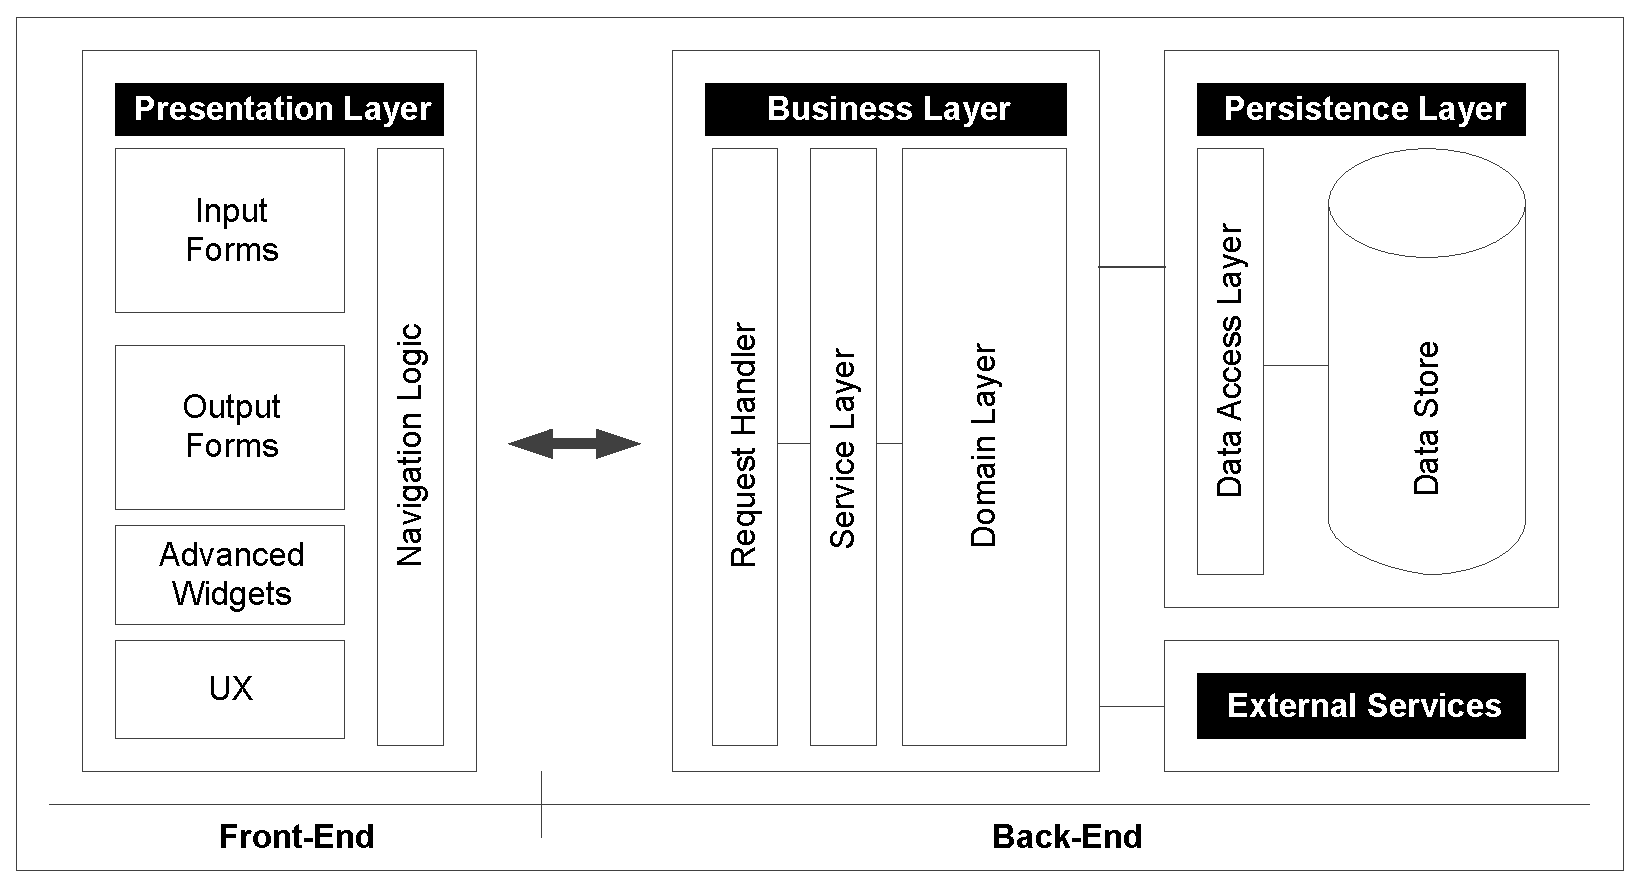
\includegraphics[width=\linewidth]{images/intro/enterpriseArchitectures00.eps}
            }
        }
        \only<1|handout:0>{
            \rput[lt](0,0){
                \includegraphics[width=\linewidth]{images/intro/enterpriseArchitectures01.eps}
            }
    \end{center}
\end{frame}

\begin{frame}[c]
	\frametitle{Responsabilidades de la Capa de Persistencia}
	\begin{enumerate}[<+->]
        \item Almacenar los datos de manera no vol�til.
        \item Recuperar datos del almac�n persistente,
        \item Asegurar la disponibilidad de los datos.
        \item Controlar la integridad de los datos.
        \item Asegurar un acceso eficiente a los datos.
	\end{enumerate}
\end{frame}

\begin{frame}[c]
    \frametitle{Tecnolog�as de Persistencia}
    \begin{description}
        \item[Relacional] Madurez, robustez y propiedades ACID.
        \item[NoSQL] Escalabilidad y rendimiento sacrificando ACID.
        \item[XML/JSON] Simplicidad.
    \end{description}
\end{frame}


\section{Puentes de Persistencia de Objetos}

\begin{frame}[c]
    \frametitle{Impedancia Objeto - Persistencia}
    \begin{block}{Impedancia Objetual}
    La \emph{impedancia objetual} se refiere al desacoplamiento que puede existir en los conceptos del paradigma orientado a objetos y el paradigma utilizado por el almac�n de persistencia.
    \end{block}
\end{frame}

\begin{frame}
    \frametitle{Impedancia Objeto - Relacional}
     %% Atributos multivaluados -
     %% Asociaciones            -
     %% Navegabilidad           -
     %% Herencia                -
     %% Evitar joins            -
\end{frame}


\begin{frame}
    \frametitle{Puentes de Persistencia de Objetos}
    %% Imagen con el esquema de persistencia
\end{frame}

\section{Patrones Estructurales}

\section{Patrones de Acceso a Datos}

%% DAO

%% Repository

%% Unit of Work

%% Identity Map

%% Lazy Load

\section{Patrones de Control de la Concurrencia}

\section{Java Persistence API}

\section{Spring Data}

\section{Sumario y Conclusiones}

\end{document}
